%\documentclass[12pt]{report} %you must choose a document class

%\documentclass[12pt]{letter}
%\signature{Your name}
%\address{Street \\ City \\ Country}
%\begin{document}
%\begin{letter}{Company name \\ Street\\ City\\ Country}
%\opening{Dear Sir or Madam:}
%\dots
%\closing{Yours Faithfully,}
%\ps{P.S. Here goes your ps.}
%\encl{Enclosures.}
%\end{letter}
%\end{document}

\pdfminorversion=7  % Used to prevent pdfpages package import warnings
\documentclass[12pt]{letter}
\signature{}
\address{Street \\ City \\ Country}


%---------------------------------------------------------------------------
% Font, Typefaces and languages
%---------------------------------------------------------------------------
\usepackage[utf8]{inputenc}
\usepackage[italian]{babel}
%\usepackage[T1]{fontenc}

%\usepackage{fontspec}
%\setmainfont{Ubuntu}
%\usepackage{fontspec}
%\setmainfont{Ubuntu Mono}
%\usepackage{kantlipsum}

%---------------------------------------------------------------------------
% Utilities
%---------------------------------------------------------------------------

% Allows use of postscript graphics and color output
\usepackage{color,graphicx} 
\textwidth 170mm
\textheight 225mm
\topmargin -15.0mm
\oddsidemargin 0mm
\evensidemargin 0mm
\parindent 0pt

\usepackage{hyperref} % Allows hyper referencing
\usepackage{pdfpages}	% Allows including externarl pdf(s)
\usepackage{tabularx} % Allows tables

% Use fancyhdr to remove ruler and add footer note
\usepackage{fancyhdr}
\usepackage{lastpage}
\pagestyle{fancy}
\fancyhf{}
\renewcommand{\headrulewidth}{0pt}
\cfoot{Pagina \thepage \hspace{1pt} di \pageref*{LastPage}}

% Create Box - v-box -  x-box
\usepackage{enumitem,amssymb}
\newlist{todolist}{itemize}{2}
\setlist[todolist]{label=$\square$}
\usepackage{pifont}
\newcommand{\cmark}{\ding{51}}%
\newcommand{\xmark}{\ding{55}}%
\newcommand{\done}{\rlap{$\square$}{\raisebox{2pt}{\large\hspace{1pt}\cmark}}%
\hspace{-2.5pt}}
\newcommand{\wontfix}{\rlap{$\square$}{\large\hspace{1pt}\xmark}}


%---------------------------------------------------------------------------
% Use .csv file for data entry
%---------------------------------------------------------------------------

% csv file structure definition w/ variables name 
%\def\chopline#1;#2;#3;#4;#5;#6;#7 \\{
%\def\scuola{#1}
%\def\indirizzo{#2}
%\def\civico{#3}
%\def\comune{#4}
%\def\cap{#5}
%\def\provincia{#6}
%\def\codice{#7}
%}

% NB: only 9 parameters accepted!
\def\chopline#1;#2;#3;#4;#5;#6;#7;#8;#9 \\{
\def\Provincia{#1}
\def\Codice{#2}
\def\Tipologia{#3}
\def\Denominazione{#4}
\def\Indirizzo{#5}
\def\Civico{#6}
\def\Comune{#7}
\def\CAP{#8}
\def\IndirizzoPECAutonomia{#9}
}

%\def\chopline#1;#2;#3;#4;#5;#6;#7;#8;#9;#10;#11;#12;#13;#14;#15;#16;#17;#18;#19;#20;#21;#22;#23;#24;#25;#26;#27;#28;#29;#30;#31;#32;#33;#34;#35;#36;#37;#38;#39;#40;#41 \\{
%\def\Provincia{#1}
%\def\Codice{#2}
%\def\Tipologia{#3}
%\def\Denominazione{#4}
%\def\Indirizzo{#5}
%\def\Civico{#6}
%\def\Localita{#7}
%\def\CodComune{#8}
%\def\Comune{#9}
%\def\CAP{#10}
%\def\Distr{#11}
%\def\Telefono{#12}
%\def\CaratteristicaScuola{#13}
%\def\SedeDirettivo{#14}
%\def\CodiceSedeRiferimento{#15}
%\def\CodiceSedeDirettivo{#16}
%\def\DenominazioneSedeDirettivo{#17}
%\def\IndirizzoSedeDirettivo{#18}
%\def\CodComuneSedeDirettivo{#19}
%\def\ComuneSedeDirettivo{#20}
%\def\CAPSedeDirettivo{#21}
%\def\DistrSedeDirettivo{#22}
%\def\ClassificazioneAutonomia{#23}
%\def\OrganicoAutonomia{#24}
%\def\OrganicoSede{#25}
%\def\NumSediAutonomia{#26}
%\def\MacrotipologiaAutonomia{#27}
%\def\TipologiaAutonomia{#28}
%\def\TipologiaSede{#29}
%\def\SComuneMontano{#30}
%\def\TelefonoSedeAutonomia{#31}
%\def\FaxSedeAutonomia{#32}
%\def\FaxSedeAutonomiaAlt{#33}
%\def\IndirizzoMailAutonomia{#34}
%\def\IndirizzoMailSedeCorsi{#35}
%\def\IndirizzoPECAutonomia{#36}
%\def\IndirizzoPECSedeCorsi{#37}
%\def\CodiceISTATcomuneSede{#38}
%\def\coorY{#39}
%\def\coorX{#40}
%\def\location{#41}
%}


% Retrive data from csv and rows loop.
% NB:  --enable-write18 should be active in the
% (La)TeX compiler command line argument
\ifx\conditionmacro\undefined
  \newread\data
  \openin\data=Licei_scelti_9COL.csv
  \loop
    \read\data to \line
  \unless\ifeof\data
    \expandafter\chopline\line\\
    \immediate\write18{%
    pdflatex --jobname="\jobname_\Codice"
    "\gdef\string\conditionmacro{\line}\string\input{\jobname}"
    }%
  \repeat
  \closein\data
  \expandafter\stop
\fi
\expandafter\chopline\conditionmacro\\



\begin{document}
\begin{letter}{Company name \\ Street\\ City\\ Country}
\pagenumbering{arabic}

\begin{center}
\large \bf
DOMANDA DI MESSA A DISPOSIZIONE
\vspace{5 mm}
\end{center}

\normalsize

\begin{flushright}
Al Dirigente Scolastico \\
dell'istituzione scolastica \textbf{\Denominazione} \\
\Indirizzo,\space\Civico\space - \CAP\space\Comune\space (\Provincia) \\
Codice \Codice\space - PEC \href{mailto:\IndirizzoPECAutonomia}{\IndirizzoPECAutonomia} \\
\end{flushright}

\vspace{7 mm}

\begin{tabularx}{\textwidth}{>{\bfseries} lX }
Oggetto: & \textbf{domanda di messa a disposizione per supplenze di docente per l’a.s. 2020-2021.}
\end{tabularx}

\vspace{7 mm}

Il sottoscritto \textbf{Stefano Caglio} \hfill nato a Monza (MB) \hfill il giorno 08/10/1981 \\
residente a \hfill Monza (MB) \hfill in via Col di Lana 19\hspace{10 mm} C.F.: CGL\,SFN\,81\,R\,08\,F704\,H \\
tel: +39 333 37\,57\,003 \hfill email: \href{mailto:stefano.caglio@gmail.com}{stefano.caglio@gmail.com} \hfill PEC: \href{mailto:info@pec.stefanocaglio.com}{info@pec.stefanocaglio.com} \\

presenta domanda di messa a disposizione in caso di esaurimento delle graduatorie d'istituto per le seguenti tipologie di posto e/o classi di concorso:

  %\item Immediate plan of action.
\begin{todolist}[itemsep=0pt,parsep=0pt]
  \item per posti di scuola dell'infanzia;
  \item per posti della scuola primaria;
	\item[\done] per le seguenti classi di concorso della scuola secondaria di I e II grado:
		\begin{itemize}[itemsep=0pt,parsep=0pt]
			\item A-20 (ex A038 A049) - Fisica [14 cfu mancanti in FIS/01]
			\item A-26 (ex A047 A049) - Matematica [47.5 cfu mancanti in MAT/02, MAT/03, MAT\-/05, MAT/06, MAT/08]
			\item A-36 - Scienze e tecnologie della logistica
			\item A-38 (ex A001) - Scienze e tecnologie delle costruzioni aeronautiche
			\item A-41 (ex A042) - Scienze e tecnologie informatiche
			\item A-42 (ex A020) - Scienze e tecnologie meccaniche
			\item A-47 (ex A048 A049) - Scienze matematiche applicate
		\end{itemize}
	\item Posti di insegnamento ad alunni disabili della scuola (senza titolo di Sostegno): \\
				$\square$ infanzia \hfill $\square$ primaria \hfill $\square$ secondaria di I grado  \hfill $\square$ secondaria di II grado
\end{todolist}


A tale scopo, consapevole delle sanzioni penali in caso di dichiarazioni non veritiere, di formazione o di uso di atti falsi, richiamate dall'art. 76 del D.P.R. 445 del 28/12/2000 n. 445 così come modificato e integrato dell'art. 15 della Legge 16/01/2003 n.3 
\begin{center}
\textbf{D I C H I A R A}
\end{center}

%\begin{itemize}
  %\item Immediate plan of action.
  %\begin{todolist}
  %\item[\done] Frame the problem
  %\item Write solution
  %\item[\wontfix] profit
  %\end{todolist}
%\end{itemize}

\begin{todolist}[itemsep=1pt,parsep=0pt]
  \item[\done] di essere cittadino italiano;
	\item[\done] di godere dei diritti civili e politici; 
	\item[\done] di essere nella seguente posizione agli effetti e adempimenti degli obblighi militari: dispensato ai sensi della legge 226/2004;
	\item[\done] di non aver riportato condanne penali e di non essere destinatario di provvedimenti che riguardano l’applicazione di misure di prevenzione, di decisioni civili e di provvedimenti amministrativi iscritti nel casellario giudiziale ai sensi della normativa vigente;
	\item[\done] di non essere sottoposto a procedimenti penali;
	\item[\done] di possedere il seguente titolo di studio: Laurea Specialistica in Ingegneria Aerospaziale (D.M. 509/99 - classe 25/S) conseguito il 23/12/2009 presso Politecnico di Milano e che nel proprio piano di studio sono stati superati gli esami necessari per accedere alle classi di concorso  della scuola secondaria sopra riportate;
	\item di essere in possesso dei 24 CFU conseguiti il \dotfill A.A. \dotfill / \dotfill presso \dotfill;
	\item di essere in possesso della certificazione lingua inglese: \hfill $\square$ B2 \hfill $\square$ C1 \hfill $\square$ C2 \\
	conseguita il \dotfill presso l'Ente Certificatore \dotfill;
	\item[\done] di essere in possesso della certificazione informatica: \\
	\done Lim \hfill \done Tablet \hfill $\square$ Animatore Digitale \hfill \done Coding scuola secondaria \hfill \done IT security \\
	conseguite fra il 01/12/2020 e il 14/12/2020 presso l'Ente Certificatore EIPASS;
	\item di essere in possesso del titolo di specializzazione per l'insegnamento ad alunni disabili nella tipologia di scuola indicata in precedenza, conseguito il \dotfill presso \dotfill;
	\item di essere in possesso dei seguenti titoli di insegnamento didattico differenziato nella scuola primaria: \hspace{0.8cm} $\square$ Montessori \hspace{0.8cm} $\square$ Pizzigoni \hspace{0.8cm} $\square$ Agazzi
	\item[\done] di prestare il proprio consenso al trattamento dei dati personali ai sensi del Regolamento 2016/679/UE del Parlamento europeo e del Consiglio, del 27 aprile 2016, relativo alla protezione delle persone fisiche con riguardo al trattamento dei dati personali, nonché alla libera circolazione di tali dati, che abroga la direttiva 95/46/CE (regolamento generale sulla protezione dei dati), e del decreto legislativo 30 giugno 2003, n. 196.
\end{todolist}

\vspace{10 mm}

Monza, \today

%Monza, \today \hspace{6cm} Firma
%
%\vspace{25 mm}
%
%\begin{tabularx}{\textwidth}{>{\bfseries} lX }
%Allegati: & Curriculum Vit\ae \\
%& Copia carta d'identità
%\end{tabularx}


\closing{%Firma:\\
\fromsig{
\includegraphics[scale=0.65]{signature.png}} \\
\fromname{Stefano Caglio}
}
\encl{Curriculum Vit\ae \\
			Copia carta d'identità}


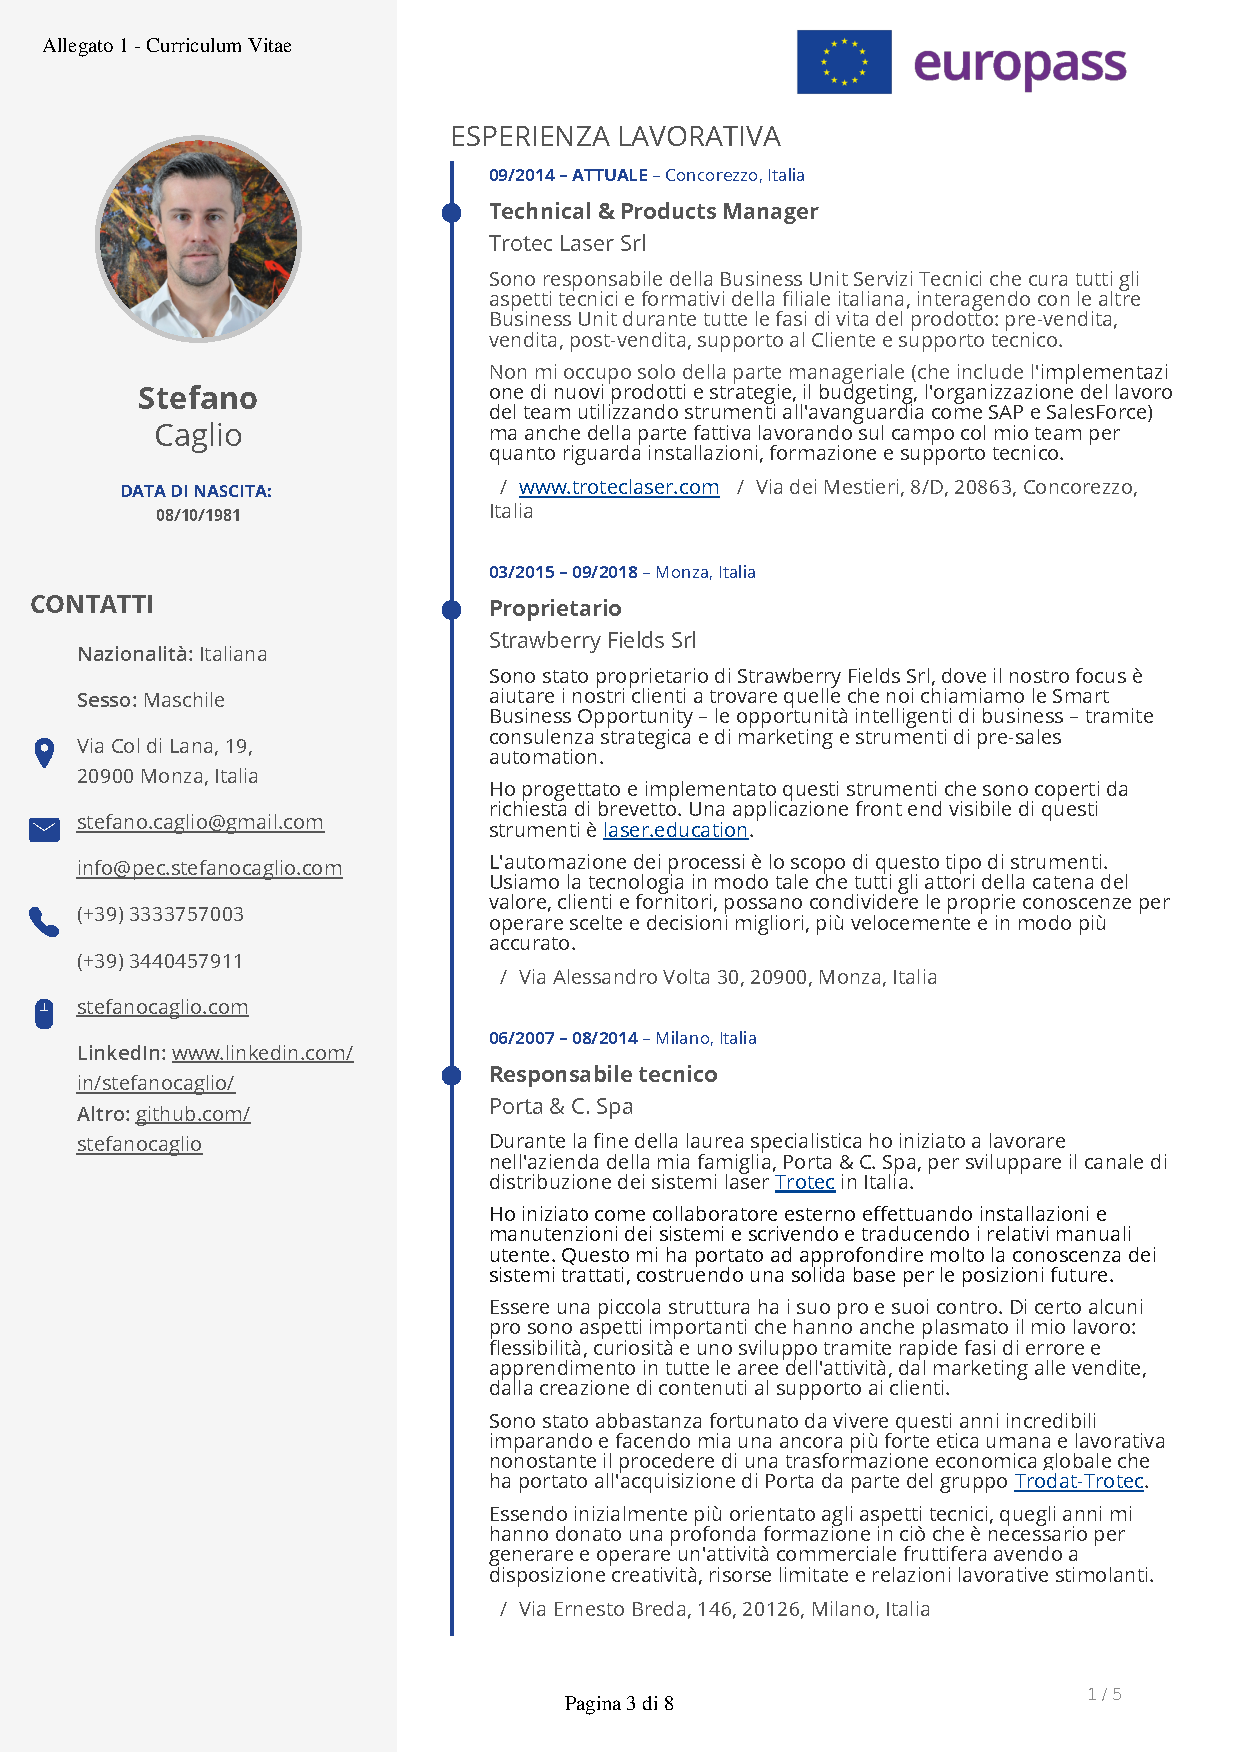
\includepdf[pages=-]{Allegato1_CV_Caglio}
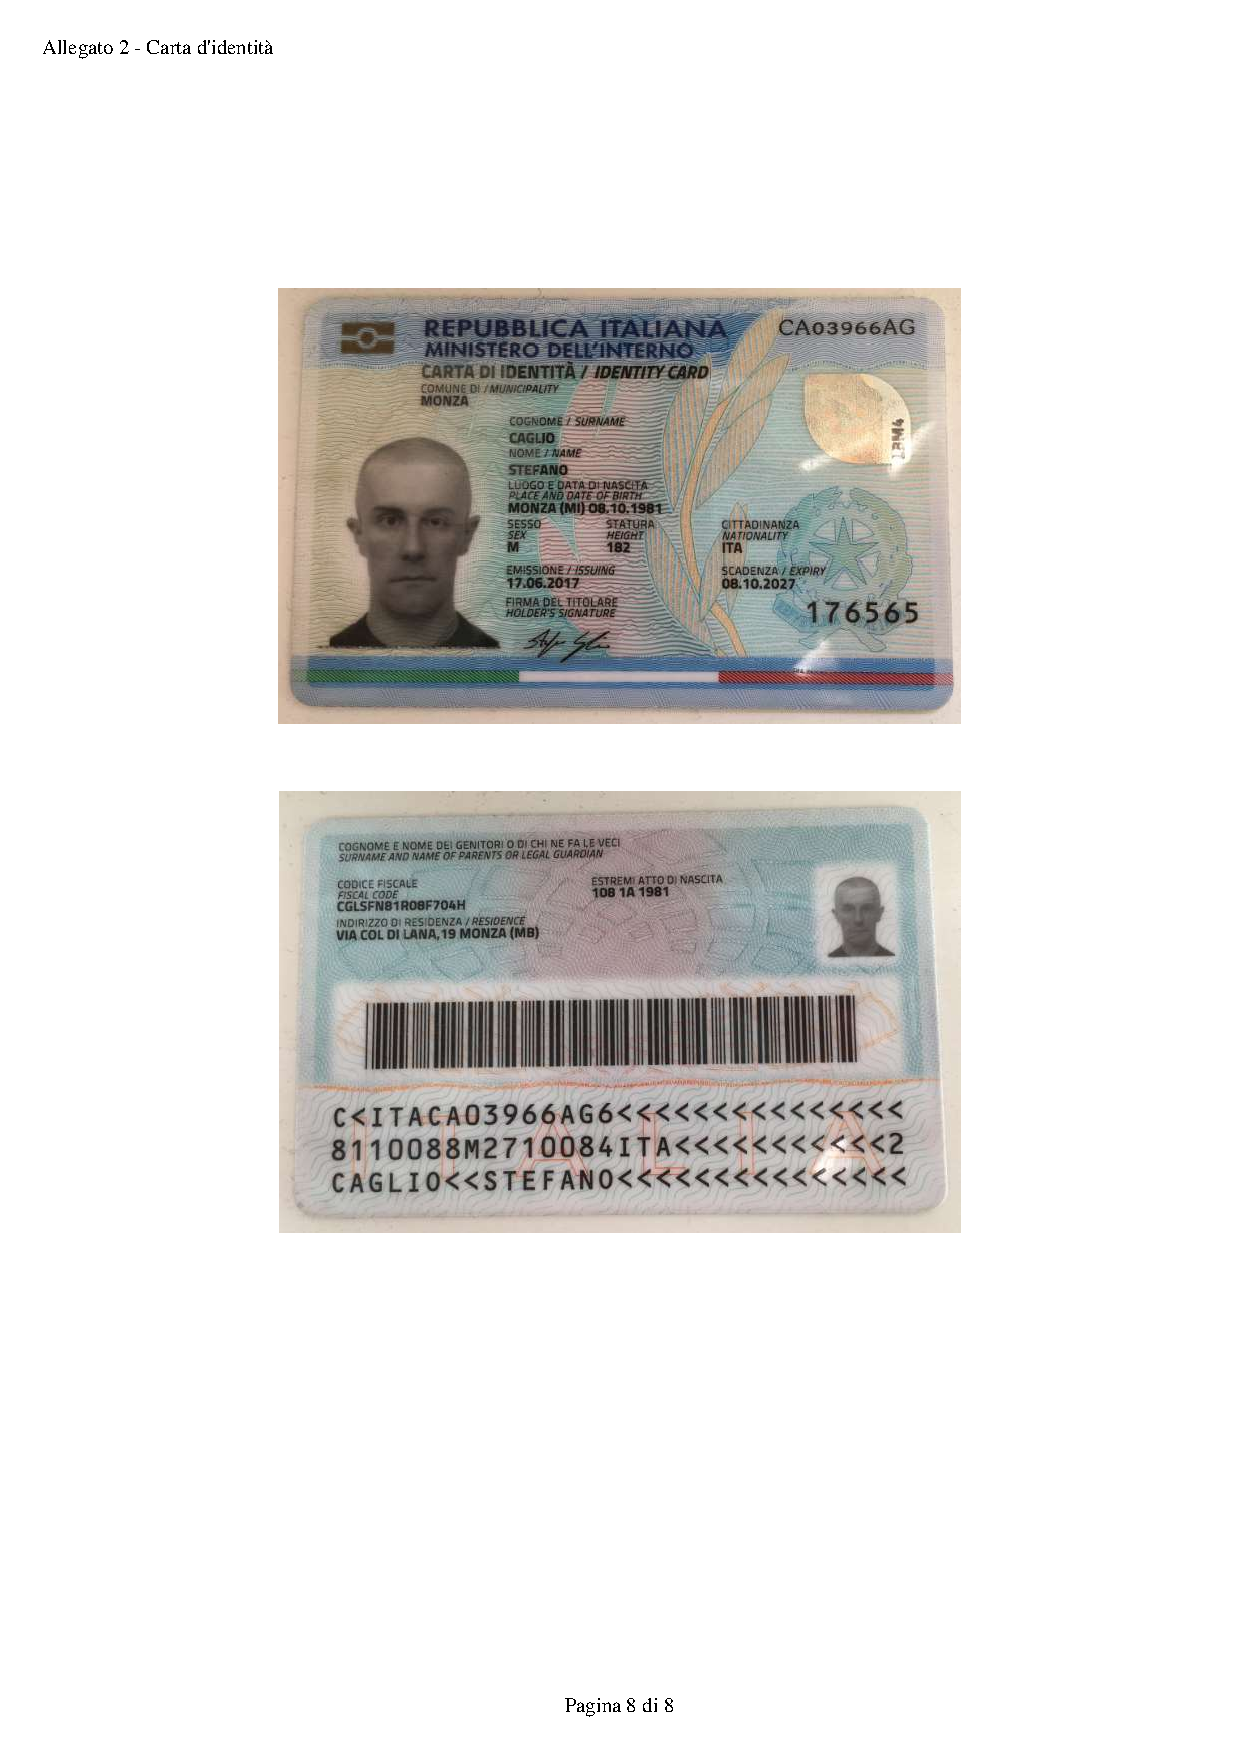
\includepdf[pages=-]{Allegato2_CI_Caglio}

\end{letter}
\end{document}

